%%%% Weekly Report Information %%%%
\newcommand{\handoutName}{Weekly report}
\newcommand{\handoutdate}{\today}
%\newcommand{\duedate}{}
\input{Header.tex}

\section{My \emph{Objectives} this week}
\begin{itemize}
\item Completing the successful runs for the object manipulation experiment.
\item Making a new plot for pure torque control.
\item Friction idea: if it works and have a demonstration of that.

\end{itemize}
\section{My \emph{Accomplishments} this week}


\begin{itemize}
\item The block pushing experiment worked! We had 4 more successful runs. They took in average 45 minutes to accomplish each.
\item We had the pure torque control experiment. Attached is the plot.
\item Mable tested if the magnets are good enough for the covariance control, and she said they are.
\item Started writing the algorithms.
\item Mable worked on the simulation, but it doesn't work yet. 
\item Lillian wrote the object orientation control base code.
\end{itemize}

\begin{figure}[h]
\begin{center}
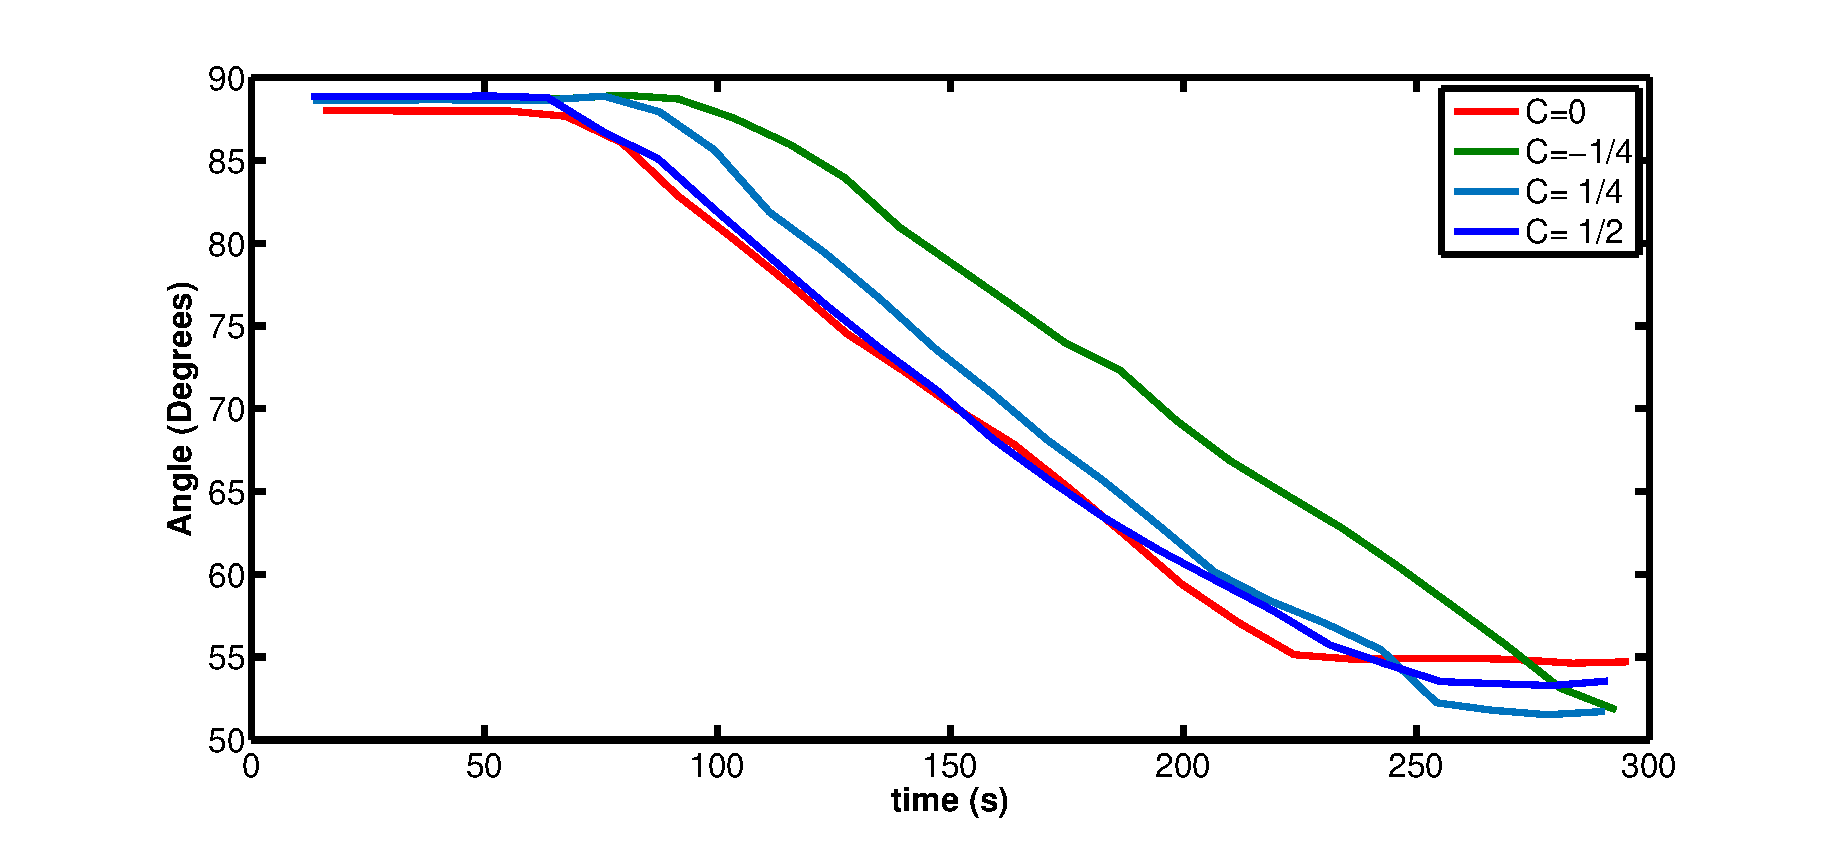
\includegraphics[width=\columnwidth]{JulyTorqueControlAll}
\caption{Four different CLs to find the best. Here you see that the one with the lowest was affecting the object for the whole 5 minutes.}
\end{center}
\end{figure}


\section{My \emph{Plan} for next week}

\begin{itemize}
\item We will have a manual control for the covariance control.
\item The simulation still doesn't work completely. I would work on it a little bit to make it work.
\item Object orientation control needs some ideas to work. It doesn't work when robots are in a good position.
\end{itemize}

\subsection{Meeting with Dr. Becker  }

\begin{itemize}
\item You are not here for the next meeting!
\end{itemize}

\end{document}
